\section{Servidor de ficheiros}

No servidor de ficheiros é possível a integração com a interface de gestão do \emph{Central Management} que agiliza a configuração das principais funcionalidades deste serviço.

No separador \emph{ETFS} é possível aceder a seguinte interface.

\begin{figure}[H]
    \begin{center}
    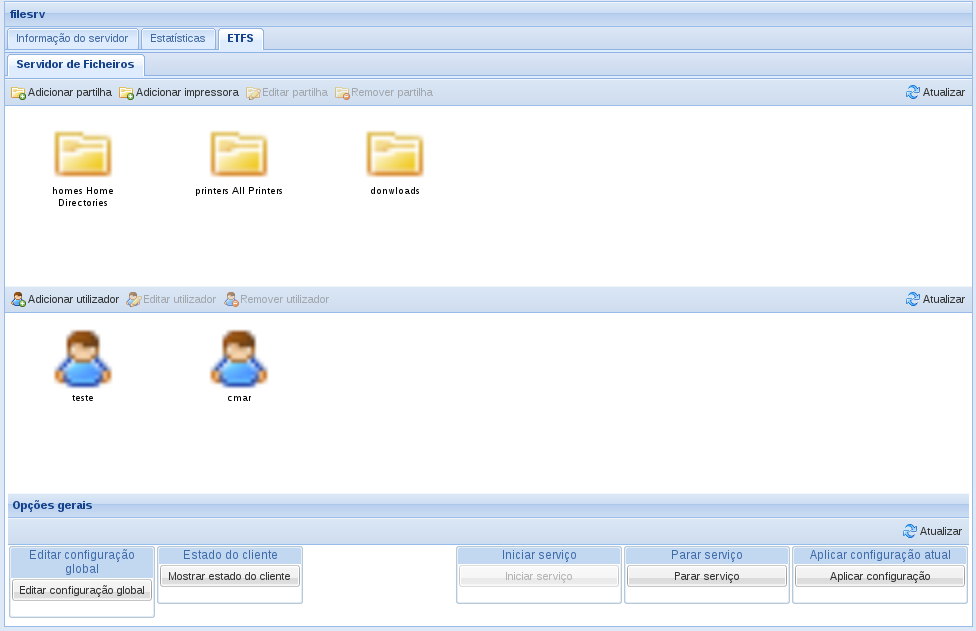
\includegraphics[scale=0.38]{screenshots/etfs/etfs_main.png}
    \caption{Interface de gestão do servidor de ficheiros}
    \label{fig:etfs_main}
    \end{center}
\end{figure}

Nesta interface podemos fazer as várias tarefas de gestão do servidor de ficheiros, tais como, aceder à configuração geral, iniciar e/ou parar serviço, gerir as partilhas e os utilizadores e consultar estado das ligações e serviço.

\begin{figure}[H]
    \begin{center}
    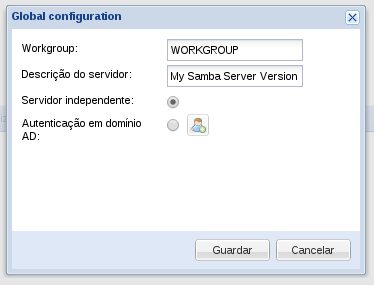
\includegraphics[scale=0.38]{screenshots/etfs/etfs_edit_global_config_user.png}
    \caption{Editar configuração global}
    \label{fig:etfs_global_config_user}
    \end{center}
\end{figure}

Ao editar a configuração global é necessário definir o \emph{Workgroup}, opcionalmente, uma descrição e definir o tipo de configuração: Servidor independente ou com autenticação em domínio \emph{Active Directory}.

No primeiro caso, o serviço comporta-se como o servidor com autenticação local e onde é possível definir os utilizadores na interface.

No segundo caso, o servidor é agregado a um domínio onde é efectuada a autenticação dos utilizadores. Toda a parte de gestão de utilizador é feita na \emph{Active Directory}.

\begin{figure}[H]
    \begin{center}
    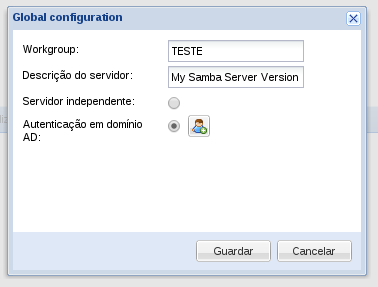
\includegraphics[scale=0.38]{screenshots/etfs/etfs_edit_global_config_ad.png}
    \caption{Editar configuração global com autenticação na AD}
    \label{fig:etfs_edit_global_config_ad}
    \end{center}
\end{figure}

Para definir a configuração de servidor com autenticação no domínio \emph{Active Directory}, é necessário adicionar o servidor ao domínio.
E, para isso, é necessário proceder á configuração do domínio, servidor de \emph{Active Directory} e nome e password de administrador de domínio tal como apresentado na figura \ref{fig:etfs_join_to_ad}.

\begin{figure}[H]
    \begin{center}
    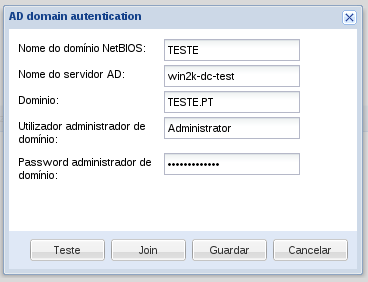
\includegraphics[scale=0.38]{screenshots/etfs/etfs_join_to_ad.png}
    \caption{Configuração de autenticação no domínio da AD}
    \label{fig:etfs_join_to_ad}
    \end{center}
\end{figure}

Depois de efectuada a configuração global do servidor de ficheiros, é possível efectuar a gestão das partilhas de ficheiros e impressoras e gestão de utilizador.

\begin{figure}[H]
    \begin{center}
    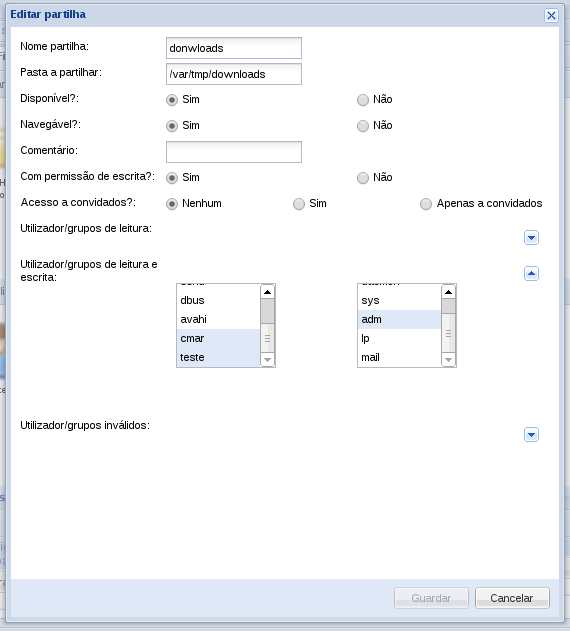
\includegraphics[scale=0.38]{screenshots/etfs/etfs_edit_file_share.png}
    \caption{Criar/editar partilha de ficheiros}
    \label{fig:etfs_edit_file_share}
    \end{center}
\end{figure}

\begin{figure}[H]
    \begin{center}
    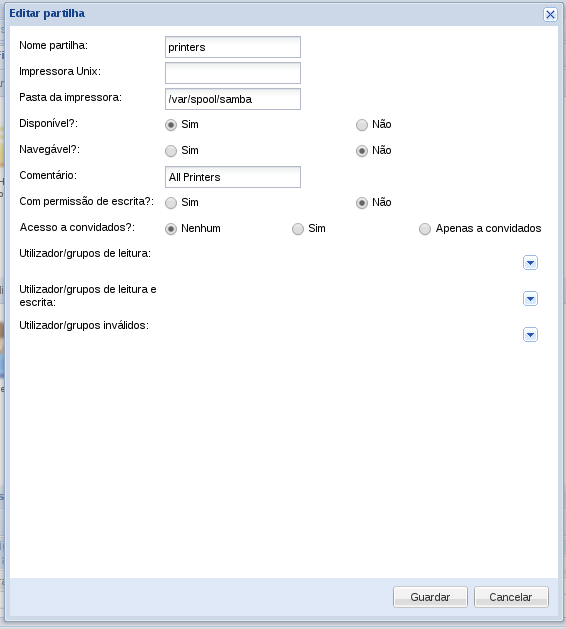
\includegraphics[scale=0.38]{screenshots/etfs/etfs_edit_printer_share.png}
    \caption{Criar/editar impressora partilhada}
    \label{fig:etfs_edit_printer_share}
    \end{center}
\end{figure}

\begin{figure}[H]
    \begin{center}
    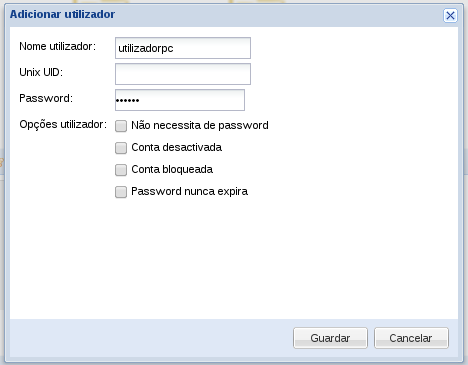
\includegraphics[scale=0.38]{screenshots/etfs/etfs_edit_user.png}
    \caption{Criar/editar utilizador}
    \label{fig:etfs_edit_user}
    \end{center}
\end{figure}

Neste interface de gestão de servidor de ficheiros é possível ainda ceder à informação sobre o estado das ligação de cada utilizador e respectiva pasta utilizada.

\begin{figure}[H]
    \begin{center}
    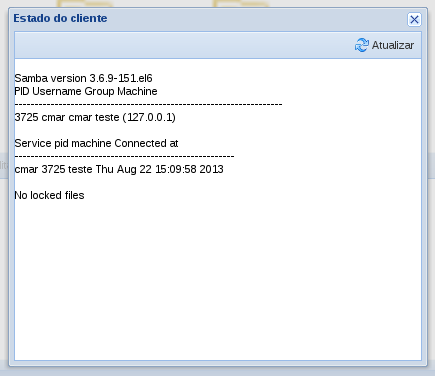
\includegraphics[scale=0.38]{screenshots/etfs/etfs_client_status.png}
    \caption{Informação sobre estado das ligações dos clientes}
    \label{fig:etfs_client_status}
    \end{center}
\end{figure}

